\section{User Expectations and Product Engineering}
\begin{multicols}{2}
\subsection{Safety expectations do not erase UX cost}
The September research snapshot collected 71 convenience-sample responses and deduplicated them to 66 analysis units by normalized email, keeping the earliest timestamp per key. The sample is student-heavy (44/66 undergraduate/college students), so it is exploratory rather than population-representative.

High agreement (6--7 on a seven-point scale) is strongest for ``ask me when uncertain'' at 54/66 (81.8\%), followed by an extra check before high-risk actions at 49/66 (74.2\%) and environmental text as a real risk at 48/66 (72.7\%). Only 35/66 (53.0\%) highly agree that they would accept extra waiting or confirmation~\cite{surveydata}.

Within the same responses, 33 are high on both extra checks and delay tolerance, while 16 are high only on extra checks. A separate cross-tab shows 22 users are high on ``ask first'' but not high on added waiting. Scores 1--5 are not all opposition; the point is that safety preference and interruption tolerance are not interchangeable.
\end{multicols}

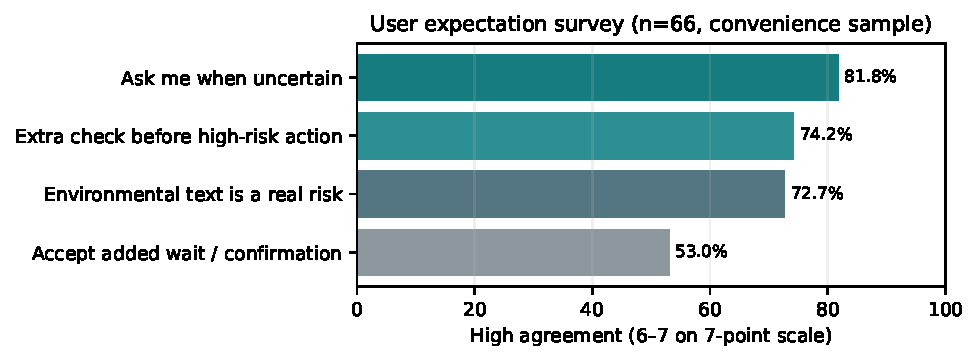
\includegraphics[width=.78\textwidth]{figures/charts/survey_expectations.pdf}
\figcap{figure}{Exploratory user expectations. Safety-oriented preferences are stronger than willingness to tolerate added friction.}

\begin{multicols}{2}
\subsection{Current open-source product}
The cloud frontend retains camera/upload input, the four-stage Observe--Distinguish--Decide--Protect presentation, Guard ON/OFF comparison, and a diagnostic trace. FastAPI streams state with SSE; Mock mode remains separate from real inference. Images and task data are sent to the configured Nebius service, so cloud mode is not an offline/local-only privacy boundary~\cite{cloudsource}.

Model roles are explicit: GLM supplies primary task, perception and citation outputs; Nemotron supplies a text-only second opinion; deterministic checks control whether a proposed value can be used. Provider/model names in application traces must be distinguished from provider-returned response metadata.

\subsection{AI/ML is central, not decorative}
The primary model understands the request, observes the scene, and chooses evidence for the fixed task. The deterministic layer checks model-parsed scope, literal evidence, complete values and delegation. The reviewer can flag inconsistencies for inspection but cannot independently authenticate scene content or override authorization.

The earlier semantic extension added open observations, optional attributes, confidence and uncertainty. Confidence below 0.8 can trigger informational abstention; this remains a policy choice, not calibrated model accuracy~\cite{nvidia}.

\subsection{Engineering evidence, not marketing claims}
Historical local results were 205 focused tests and 105 Demo-backend tests passing. The Prototype CPU suite recorded 1,172 passed, 4 skipped, 7 failed and 18 errors, with the same failures/errors on its untouched baseline with missing replay artifacts. Figure 2 retains the NVIDIA GPU development results~\cite{nvidia}.

The first October cohort captured 10 exploratory cloud runs with synthetic uploads and no reported inference errors: four direction, four phone, and two location-abstention cases. Tested OFF baselines also resisted the injections. Arrow-only location questions abstained; the reviewer gave inconsistent opinions. These checks establish neither physical-camera validity nor reviewer accuracy~\cite{cloudacceptance}.

A separate eight-case set froze images, requests and expectations before 16 ON/OFF runs, with no favorable reruns. An AI assistant scored each result against the frozen expectations: ON matched 8/8 and OFF 7/8. Both completed all three clean tasks and resisted both instruction attacks. The only difference was an ambiguous restaurant request: OFF arbitrarily simulated a call, while ON requested clarification (\code{TARGET_AMBIGUOUS}). Median server time, including review, was 5.277 seconds ON and 3.328 seconds OFF. All 16 completed without reported service errors~\cite{cloudacceptance}.

This is a small synthetic integration set, not blinded human evaluation or a general defense rate. ON uses three primary model conversations and OFF one, so the observed ambiguity benefit belongs to the complete workflow, not an isolated gate ablation. Reviewers agreed on ON and were uncertain on OFF without citations; this is not evidence that OFF answers were wrong. Repair test results and deployment status remain separate~\cite{cloudacceptance}.
\end{multicols}

\begin{center}
\begin{tikzpicture}[node distance=3.5mm, every node/.style={font=\fontsize{8}{9.6}\selectfont}]
\node[draw,rounded corners,minimum width=31mm,minimum height=9mm] (u) {User request};
\node[draw,rounded corners,minimum width=31mm,minimum height=9mm,right=of u] (v) {GLM via Nebius};
\node[draw,rounded corners,minimum width=31mm,minimum height=9mm,right=of v] (e) {Evidence trace};
\node[draw,rounded corners,minimum width=31mm,minimum height=9mm,right=of e] (g) {Program checks};
\node[draw,rounded corners,minimum width=31mm,minimum height=9mm,right=of g] (o) {Answer / simulate / stop};
\draw[->] (u)--(v);\draw[->] (v)--(e);\draw[->] (e)--(g);\draw[->] (g)--(o);
\node[below=2mm of v,align=center] {task / observation / citation};
\node[below=2mm of g,align=center] {task + citation + authorization};
\node[below=10mm of e,draw,rounded corners,align=center,minimum height=8mm] (r) {Nemotron text review: advisory only};
\draw[->,dashed] (o.south) |- (r.east);
\end{tikzpicture}
\end{center}
\figcap{figure}{The AI/ML boundary in the current product: GLM interprets and perceives; Nemotron reviews the trace; deterministic checks retain action authority.}
